\section{Logic Network Representation}\label{cha:networkRepresentation}

Logic networks are graphical models with an interpretation by propositional logics.
We first distinguish between Markov Logic Networks, which are an approach to soft logics in the framework of exponential families, and Hard Logic Networks, which correspond with propositional knowledge bases.
Then we exploit non-trivial boolean base measures to unify both approaches by Hybrid Logic Networks, which are itself in exponential families.




%Markov Logic Networks are probability functions of truth assignments to logical functions.
%They respect propositional logic as hard constraints, but have beyond that freedom to shape probability distributions on possible situations.
%To capture these properties, we define them as graphical models with structure cores representing propositional logics and activation cores representing the specification of probability distributions.
% We in this part employ them to combine the probabilistic and the logical paradigm.


\subsection{Markov Logic Networks}

Markov Logic Networks exploit the efficiency and interpretability of logical calculus as well as the expressivity of graphical models. 

\subsubsection{Markov Logic Networks as Exponential Families}

We introduce Markov Logic Networks in the formalism of exponential families (see \secref{sec:exponentialFamilies}).

\begin{definition}[Markov Logic Networks]
	Markov Logic Networks are exponential families $\mlnexpfamily$ with sufficient statistics by functions
		\[ \mlnstat : \atomstates \rightarrow \bigtimes_{\exformulain}[2] \subset \rr^{\cardof{\formulaset}} \]
	defined coordinatewise by propositional formulas $\exformulain$.
\end{definition}

% Binary Statistics as propositional formula
Since the image of each feature is contained in $[2]$, they are propositional formulas (see Def.~\ref{def:formulas}).

% Characterization of MLNs among exponential families: When choosing binary features
Conversely, any binary feature $\sstatcoordinateof{\selindex}$ of an exponential family defines a propositional formula (see \defref{def:formulas}).
Thus, any exponential family of distributions of $\atomstates$, such that $\imageof{\sstatcoordinateof{\selindex}}\subset\ozset$ for all $\selindexin$ is a set of Markov Logic Networks with fixed formulas.

% Formula Selecting Networks
%We will further study the sparse representation of formula sets in \charef{cha:architectures}.


The sufficient statistics consistent in a map $\formulaset$ of formulas brings the following advantages:
\begin{itemize}
	\item Numerical Advantage: The sufficient statistics is decomposable into logical connectives. 
	If the formulas are sparse (in the sense of limited number of connectives necessary in their representation), this gives rise to efficient tensor network decompositions of the relational encoding.
	\item Statistical Advantage: Since each formula is Boolean valued, the coordinates of the sufficient statistic are Bernoulli variables. 
	Due to their boundedness, they and their averages (by Hoeffdings inequality) are sub-Gaussian variables with favorable concentration properties (absence of heavy tails).
\end{itemize}


\begin{remark}[Alternative Definitions]
	We here defined MLNs on propositional logic, while originally they are defined in FOL.
	The relation of both frameworks will be discussed further in \charef{cha:folModels}.
\end{remark}



\subsubsection{Tensor Network Representation}

Based on the previous discussion on the representation of exponential families by tensor networks in \secref{sec:exponentialFamilies} we now derive a representation for Markov Logic Networks.

\begin{theorem}[Relational Encodings for Markov Logic Networks]\label{the:mlnTensorRep}
	A Markov Logic Network to a set of formulas $\formulaset = \{\enumformula \, : \, \selindexin\}$ is represented as
	\begin{align*}
		\mlnprobat{\shortcatvariables} = 
		\normationof{\{\enumformulaccwith : \selindexin \} \cup \{\enumformulaacwith : \selindexin \}
		}{\shortcatvariables}
	\end{align*}
	where we denote for each $\selindexin$ an activation core
	\begin{align*}
		\enumformulaacwith
		= \begin{bmatrix} 1 \\
		 \expof{\canparamat{\indexedselvariable}} 
		 \end{bmatrix}[\enumformulavar] \, .
	\end{align*}
\end{theorem}
\begin{proof}
	The claim follows from Theorem~\ref{def:expFamilyTensorRep} and the following contraction equations.
	We have with the grouped variable $\headvariableof{\formulaset} = \{\enumformulavar\, : \, \selindexin\}$
	\begin{align*}
		\rencodingofat{\formulaset}{\headvariableof{\formulaset},\shortcatvariables}
		= \contractionof{\{\enumformulaccwith : \selindexin \}}{\headvariableof{\formulaset},\shortcatvariables} \, .
	\end{align*}
	Since we have a Markov Logic Network we have $\imageof{\enumformula}\subset [2]$ and thus
	\begin{align*}
		\enumformulaac\left[\headvariableof{\selindex}=\headindex_{\selindex}\right]
		= \begin{cases}
			1 & \text{for} \quad \headindex_{\selindex} = 0 \\
			\expof{\canparamat{\indexedselvariable}} & \text{for} \quad \headindex_{\selindex}  = 1
		\end{cases}  
	\end{align*}
	Using these equations, the claim follows from Theorem~\ref{def:expFamilyTensorRep}.
\end{proof}

\begin{figure}[h]
\begin{center}
	\begin{tikzpicture}[thick, scale=0.35] % , baseline = -3.5pt

\drawundiratomindices{0}{-4}
\draw (-2,-1) rectangle (6, -3);
\node[anchor=center] (text) at (2,-2) {$\expof{\canparamat{\indexedselvariable}\cdot\enumformula}$};

		
\node[anchor=center] (text) at (10,-2) {${=}$};


\begin{scope}[shift={(15,-2)}]

		\draw (-0.5,3) rectangle (4.5, 5);
		\node[anchor=center] (text) at (2,4) {$\enumformulaac$};

		\drawvariabledot{2}{2.25}
		\draw[] (2,2.25) -- (2,3);
		\draw[->] (2,1) -- (2,2.5) node[midway, left] {\tiny $\headvariableof{\selindex}$};
		
		\draw (-1,1) rectangle (5, -1);
		\node[anchor=center] (text) at (2,0) {$\bencodingof{\enumformula}$};

		\drawatomindices{0}{-2}

\end{scope}

\end{tikzpicture}
\end{center}
\caption{Factor of a Markov Logic Network to a formula $\enumformula$, represented as the contraction of a computation core $\enumformulacc$ and an activation core $\enumformulaac$.
	While the computation core $\enumformulacc$ prepares based on basis calculus a categorical variable representing the value of the statistic formula $\enumformula$ dependent on assignments to the distributed variables, the activation core multiplies an exponential weight to coordinates satisfying the formula.
}
\label{fig:mlnFactor}
\end{figure}

% 
Since any member of an exponential family is a Markov Network with tensors to each coordinate of the statistic, also Markov Logic Networks are Markov Networks.

\begin{corollary}\label{cor:MLNasMN}
	Given a set $\formulaset$ of formulas on atomic variables $\catvariableof{\nodes}$, we construct a $\graph=(\nodes,\edges)$, where $\nodes$ are decorated by the atoms and
		\[ \edges = \{ \nodesof{\formula}: \formula\in\formulaset \} \, , \]
	where by $\nodesof{\formula}$ we denote the minimal set such that there exists a tensor $\hypercoreat{\catvariableof{\nodesof{\formula}}}$ with
		\[ \formulaat{\catvariableof{\nodes}} = \hypercoreat{\catvariableof{\nodesof{\formula}}} \otimes \onesat{\catvariableof{\nodes/\nodesof{\formula}}} \, . \]		
	Any Markov Logic Network $\mlnparameters$ is then a Markov Network given the graph $\graphof{\formulaset}$
	$\{\expof{\canparamat{\indexedselvariable}\cdot\enumformula}
\, :\,\selindexin\}$.
\end{corollary}


% MLN as graphical models
Markov Logic Networks are Markov Networks with the factors given in a restricted form from the weighted truth of a formula.
Each formula is seen as a factor of the graphical model.

There are two sparsity mechanisms drastically reducing the number of parameters (and loosing generality):
\begin{itemize}
	\item Factors/Formulas contain only subsets of atoms (already in Corollary~\ref{cor:MLNasMN} exploited):
		The underlying assumptions of conditional independence loss generality.
	\item Structure in the factors: In MLN each factor corresponds with a formula evaluated on possible worlds.
		Again, any possible factor can be represented by a formula, but we concentrate on small formulas (see Theorem \ref{the:FormulaToTensor}).
\end{itemize}


% 
\red{We can extend the set of variables, by including the hidden formulas, and get a Markov Network of the relational encodings of connectives and headcores.
Here hidden variables are additional variables facilitating the decomposition, but not appearing in open variables of contractions when doing reasoning.
One can then exploit redundancies and make sure that every subresult is computed just once, by dropping relational encodings with identical head functions.
}


\begin{figure}[h]
\begin{center}
	\begin{tikzpicture}[scale=0.35, thick, yscale=-1] % , baseline = -3.5pt

\draw (-5,-3) rectangle (1, -5);
\node[anchor=center] (text) at (-2,-4) {$\expof{\canparamat{0}\cdot\formulaof{0}}$};

\draw (3,-3) rectangle (9, -5);
\node[anchor=center] (text) at (6,-4) {$\expof{\canparamat{1}\cdot\formulaof{1}}$};


\draw[->] (0,1)--(0,-1)  node[midway,left] {\tiny $\catvariableof{a}$}; 
\drawvariabledot{0}{-1}
\draw[->] (0,-1) to[bend right=25] (-4,-3);
\draw[->] (0,-1) to[bend left=25] (4,-3);

\draw[->]  (2,1)--(2,-1) node[midway,right] {\tiny $\catvariableof{b}$}; 
\drawvariabledot{2}{-1}
\draw[->] (2,-1) to[bend right=25] (-2,-3);
\draw[->] (2,-1) to[bend left=25] (6,-3);

\draw[->] (4,1)--(4,-1) node[midway,right] {\tiny $\catvariableof{c}$}; 
\drawvariabledot{4}{-1}
\draw[->] (4,-1) to[bend right=25] (0,-3);
\draw[->] (4,-1) to[bend left=25] (8,-3);


\node[anchor=center] (text) at (12.5,-2) {${=}$};


\begin{scope}[shift={(20,0)}]

\draw[->] (0,1)--(0,-1)  node[midway,left] {\tiny $\catvariableof{a}$}; 
\draw[->]  (3,1)--(3,-1) node[midway,right] {\tiny $\catvariableof{b}$}; 
\draw[->] (6,1)--(6,-1) node[midway,right] {\tiny $\catvariableof{c}$}; 

	
\draw (-1,-1) rectangle (4, -3);
\node[anchor=center] (text) at (1.5,-2) {$\rencodingof{\lor}$};

\draw[->] (1.5,-3) --(1.5,-4.5) node[midway,right]{\tiny $\catvariableof{a \lor b}$};
\drawvariabledot{1.5}{-4.5}
\draw[->] (1.5,-4.5) --(1.5,-6) ;

\draw[] (1.5,-4.5) -- (0,-4.5);

\draw[]  (-7, -3.5) rectangle (0, -6.5);
\node[anchor=center,] (text) at (-3.5,-5) {$\begin{bmatrix} 
1 \\
\expof{\canparamat{0}}
\end{bmatrix}$};


\draw (5,-1) rectangle (7, -3);
\node[anchor=center] (text) at (6,-2) {$\rencodingof{\lnot}$};

\draw[->] (6,-3) --(6,-4.5) node[midway,right]{\tiny $\catvariableof{\lnot c}$};
\drawvariabledot{6}{-4.5}
\draw[->] (6,-4.5) --(6,-6);	
	
	
\draw (0.5,-6) rectangle (6.5,-8);
\node[anchor=center] (text) at (3.5,-7) {$\rencodingof{\lor}$};
	
\draw[<-] (4,-9.5) -- (4,-8) node[midway,right] {\tiny $\catvariableof{a \lor b \lor \lnot c}$};

\drawvariabledot{4}{-9.5}
\draw[] (4,-9.5) -- (2.75,-9.5);

\draw[]  (-4.25, -8.5) rectangle (2.75, -11.5);
\node[anchor=center,] (text) at (-0.75,-10) {$\begin{bmatrix} 
1 \\
\expof{\canparamat{1}}
\end{bmatrix}$};



\end{scope}

\end{tikzpicture}
\end{center}
\caption{Example of a decomposed Markov Network representation of a Markov Logic Network with formulas $\{\formulaof{0} = a\lor b, \formulaof{1} = a \lor b \lor \lnot c\}$.
	Since both formulas share the subformula $a\lor b$, their contracted factors have a representation by a connected tensor network.}
% Where $\actcoreofat{\enumformula}{\enumformulavar} =\begin{bmatrix} 1 & \expof{\weightof{\exformula}} \end{bmatrix}[\formulavar] $}
\label{fig:mlnDecRep}
\end{figure}


%\begin{theorem}[Selection encodings for Energy representation]
%	\red{More the definition of exponential families.}
%	The energy of Markov Logic Networks is the contraction
%		\[ \mlnenergy = \sbcontractionof{\sencodingof{\formulaset},\canparam}{\shortcatvariables} \, . \]
%\end{theorem}


\subsubsection{Energy tensors}

%% Tensor Representation of MLN
With the energy tensor
\begin{align}
	\mlnenergy\left[\shortcatvariables\right]
	= \sum_{\selindexin} \canparamat{\indexedselvariable} \cdot \enumformulaat{\shortcatvariables} 
	= \sbcontractionof{\sencodingofat{\formulaset}{\shortcatvariables,\selvariable},\canparamat{\selvariable}}{\shortcatvariables} 
\end{align}
the MLN is the distribution
\begin{align}
	\mlnprobat{\shortcatvariables} = \normationof{\expof{\mlnenergy}}{\shortcatvariables} \, . 
\end{align}

In case of a common structure of the formulas in a Markov Logic Network, Formula selecting networks can be applied to represent their energies.

% Energy representation
%The weighted sum of formulas is then the energy of the Markov Logic Network.
We represent the superposition of formulas as a contraction with s parameter tensor.
Given a factored parametrization of formulas $\exformula_{\selindices}$ with indices $\selindexof{\selenumerator}$ we have the superposition by the network representation:
\begin{center}
	\begin{tikzpicture}[thick, scale=0.35] % , baseline = -3.5pt

\node[anchor=east] (text) at (-3,0) {$\sum_{\parindexof{[\parorder]}\in\parstates} \canparamat{\selvariableof{[\parorder]}=\parindexof{[\parorder]}} {\exformula_{\parindexof{[\parorder]}}} \quad {=}$};

%\node[anchor=center] (text) at (0.5,-8) {$\mathrm{log}$};

%\drawatomcore{3.5}{-8}{$\rencodingof{\fselectionmap}$}
%\drawatomindices{3.5}{-12}	
%
%
%\drawatomcore{3.5}{-4}{$\canparam$}
%\drawparindices{3.5}{-8}	



\drawatomindices{0}{-4}
\draw (-1,3) rectangle (5, -3);
\node[anchor=center] (text) at (2,0) {$\rencodingof{\fselectionmap}$};

\draw[->] (2,3)--(2,5) node[midway,right] {\tiny $\catvariableof{\fselectionmap}$}; 
\draw (1,5) rectangle (3,7);
\node[anchor=center] (text) at (2,6) {$\tbasis$};

\draw[<-] (5,-2)--(7,-2) node[midway,below] {\tiny $\selvariableof{0}$}; 
\draw[<-] (5,-0.5)--(7,-0.5) node[midway,below] {\tiny $\selvariableof{1}$}; 
\node[anchor=center] (text) at (6,0.75) {$\vdots$};
\draw[<-] (5,2)--(7,2) node[midway,above] {\tiny $\selvariableof{\parorder\shortminus1}$}; 

\draw (7,3) rectangle (9,-3);
\node[anchor=center] (text) at (8,0) {$\canparam$};

\end{tikzpicture}
\end{center}


% Representation 
If the number of atoms and parameters gets large, it is important to represent the tensor ${\exformula_{\selindices}}$ efficiently in tensor network format and avoid contractions.
To avoid inefficiency issues, we also have to represent the parameter tensor $\canparam$ in a tensor network format to improve the variance of estimations (see \charef{cha:mlnConcentration}) and provide efficient numerical algorithms.

% Fail of full probability representation
However, when required to instantiate the probability distribution of a Markov Logic Network as a tensor network, we need to exponentiate and normate the energy tensor, a task for which relational encodings are required.
For such tasks, contractions of formula selecting networks are not sufficient and each formula with a nonvanishing weight needs to be instantiated as a factor tensor of a Markov Network. 






\subsubsection{Expressivity}\label{sec:MLNMaxMintermRep}

Based on Markov Logic Networks containing only maxterms and minterms (see \defref{def:clauses}), we here provide an expressivity study.
There are $2^{\atomorder}$ maxterms and $2^{\atomorder}$ minterms which are enough to represent any probability distribution as we show next.

\begin{theorem}\label{the:maximalClausesRepresentation}\label{the:mintermExpressivityMLN}
	Let there be a positive probability distribution
		 \[ \probat{\shortcatvariables} \in \bigotimes_{\atomenumeratorin}\rr^2 \, . \]
	Then the Markov Logic Network of minterms (see \defref{def:clauses})
		\[ \mintermformulaset = \{\mintermof{\atomindices} \, : \, \atomindices\in\atomstates \}\]
	with parameters %with nonzero weights at the maxterms indexed by $\atomindicesin$
		\[ \canparamat{\selvariableof{0}=\catindexof{0},\ldots,\selvariableof{\atomorder-1}=\catindexof{\atomorder-1}}% \weightof{\mintermof{\atomindices}} 
		= \ln \probat{\indexedcatvariables} \]
	coincides with $\probat{\shortcatvariables}$.

	Further, the Markov Logic Network of maxterms
		\[ \maxtermformulaset = \{\maxtermof{\atomindices} \, : \, \atomindices\in\atomstates \}\]
	with wparameters
		\[ \canparamat{\selvariableof{0}=\catindexof{0},\ldots,\selvariableof{\atomorder-1}=\catindexof{\atomorder-1}} %\weightof{\maxtermof{\atomindices}} 
		= - \ln\probat{\indexedcatvariables} \]
	coincides with $\probat{\shortcatvariables}$.
\end{theorem}
\begin{proof}
	It suffices to show, that in both cases of choosing $\formulaset$ by minterms or maxterms with the respective parameters
		\[ \mlnenergy =  \ln\probat{\shortcatvariables} \]
	and therefore
		\[ \mlnprobat{\shortcatvariables} 
		= \sbnormationof{\expof{\mlnenergy}}{\shortcatvariables} 
		=  \sbcontractionof{\expof{\mlnenergy}}{\shortcatvariables} 
		= \probat{\shortcatvariables}\, . \]
	
	In the case of minterms, we notice that for any $\atomindicesin$
		\[ \mintermof{\atomindices}[\shortcatvariables] = \onehotmapofat{\atomindices}{\shortcatvariables} \]
	and thus with the weights in the claim
		\[ \sum_{\atomindicesin} 
		\left( \ln \probat{\indexedcatvariables} \right) \cdot \mintermof{\atomindices}[\shortcatvariables]
		= \ln\probat{\shortcatvariables} \, .
		 \]

	For the maxterms we have analogously
		\[ \maxtermof{\atomindices}[\shortcatvariables] = \onesat{\shortcatvariables} - \onehotmapofat{\catindices}{\shortcatvariables} \]
	and thus that the maximal clauses coincide with the one-hot encodings of respective states.
	We thus have
	\begin{align*}
		& \sum_{\atomindicesin} 
		\left( - \ln \probat{\indexedcatvariables} \right) \cdot \maxtermof{\atomindices}[\shortcatvariables] \\
		& =
		\left(  \sum_{\nodes_0\subset [\atomorder]} 
		\left( - \ln \probat{\indexedcatvariables} \right) \cdot \onesat{\shortcatvariables} \right) \\
		& \quad + 
		\left(  \sum_{\nodes_0\subset [\atomorder]} 
		\left(  \ln \probat{\indexedcatvariables} \right) \cdot
		\onehotmapofat{\catindices}{\shortcatvariables} 
		\right) 
		 \\
		 & = \ln\probat{\shortcatvariables} + \lambda \cdot  \onesat{\shortcatvariables}\,,
	\end{align*}
	where $\lambda$ is a constant.
\end{proof}

% Redundant parametrization
In general, this representation is redundant, since any offset of the weight by $\lambda\cdot\ones$ results in the same distribution.
However, the only $\bar{\canparam}$ are multiples of $\onesat{\shortcatvariables}$.

% Comparison with previous schemes
Theorem~\ref{the:maximalClausesRepresentation} is the analogue in Markov Logic to Theorem~\ref{the:tensorToMaxMinTerms}, which shows that any binary tensor has a representation by a logical formula, to probability tensors.
Here we require positive distributions for well-defined energy tensors.


\begin{remark}[Representation of Markov Networks]
% Composition of Markov Networks
	If a probability distribution is representable as a Markov Network, we only need to activate clauses and terms, which variables are contained in factors.
	\red{Make a theorem out of that?}
\end{remark}



%\subsubsection{Examples}


\subsubsection{Distribution of independent variables}

We show next, the independent positive distributions are representable by tuning the $\atomorder$ weights of the atomic formulas and keeping all other weights zero.

\begin{theorem}\label{the:independentAtomicMLN}
	Let $\probat{\shortcatvariables}$ be a positive probability distribution, such that disjoint subsets of atoms are independent from each other.
	Then $\probat{\shortcatvariables}$ is the Markov Logic Network of atomic formulas
		\[ \atomformulaset = \{\atomicformulaof{\catenumerator} \, : \, \catenumeratorin \} \]
	and parameters
		\[ \canparamat{\selvariable=\catenumerator} 
		= \lnof{\frac{
		\contractionof{\probtensor}{\catvariableof{\catenumerator}=1}
		}{
		\contractionof{\probtensor}{\catvariableof{\catenumerator}=0}
		}} \]
%	Any distribution such that the atom satisfaction is independent from each other is reproducable by a MLN with nonzero weights only for the atomic formulas.
\end{theorem}
\begin{proof}
%	Using the independent assumptions, the probability tensor factorizes into normed vectors to each atom, with are transformed atomic formulas (leaving out the neutral ones tensors).
%	We then find a weight to each atom such that the vector is reproduced by the contraction with the activation core.
	
	By Theorem~\ref{the:independenceProductCriterion} we get a decomposition 
		\[ \probat{\shortcatvariables} = \bigotimes_{\catenumeratorin} \probofat{\catenumerator}{\catvariableof{\catenumerator}} \,  \]
	where 
		\[ \probofat{\catenumerator}{\catvariableof{\catenumerator}} = \sbcontractionof{\probtensor}{\catvariableof{\catenumerator}} \, . \]
	
	By assumption of positivity, the vector $\probofat{\catenumerator}{\catvariableof{\catenumerator}}$ is positive for each $\catenumeratorin$ and the parameter
		\[ \canparamat{\selvariable=\catenumerator} 
		= \lnof{\frac{
		\probofat{\catenumerator}{\catvariableof{\catenumerator}=1}
		}{
		\probofat{\catenumerator}{\catvariableof{\catenumerator}=0}
		}} \]
	well-defined.
	
	We then notice, that 
		\[ \expdistofat{(\{\atomicformulaof{\catenumerator}\},\canparamat{\selvariable=\catenumerator})}{\catvariableof{\catenumerator}} 
		= \probofat{\catenumerator}{\catvariableof{\catenumerator}}\]
	and therefore with the parameter vector of dimension $\seldim=\catorder$ defined as
		\[ \canparamat{\selvariable} = \sum_{\catenumeratorin} \canparamat{\selvariable=\catenumerator} \cdot \onehotmapofat{\catenumerator}{\selvariable}  \]
	we have
	\begin{align*}
	 	 \expdistofat{(\{\atomicformulaof{\catenumerator} \, : \, \catenumeratorin\},\canparam)}{\shortcatvariables} 
		& = \bigotimes_{\catenumeratorin} \expdistofat{(\{\atomicformulaof{\catenumerator}\},\canparamat{\selvariable=\catenumerator})}{\catvariableof{\catenumerator}} \\
		& = \bigotimes_{\catenumeratorin} \probofat{\catenumerator}{\catvariableof{\catenumerator}} \\
		& = \probat{\shortcatvariables} \, . 
	\end{align*}
\end{proof}

%In general, the statistic to an atomic formula measures the marginal distribution. -> To Parameter Estimation

% Failing to be positive -> Hybrid networks
In Theorem~\ref{the:independentAtomicMLN} we made the assumption of positive distributions.
If the distribution fails to be positive, we still get a decomposition into distributions of each variable, but there is at least one factor failing to be positive.
Such factors need to be treated by hybrid logic networks, that is they are base measure for an exponential family coinciding with a logical literal (see \secref{sec:hardNetworks}).

% Energy representation
All atomic formulas can be selected by a single variable selecting tensor, that is
	\[ \energytensorofat{(\{\atomicformulaof{\catenumerator} \, : \, \catenumeratorin\},\canparam)}{\shortcatvariables}
	= \sbcontractionof{\vselectionmapat{\shortcatvariables,\selvariable},\canparamat{\selvariable}}{\shortcatvariables} \, . 
	\]
	
% Holds also more generally for any formula! -> Place it earlier?
In case of negative coordiantes $\canparamat{\selvariable=\catenumerator}$ it is convenient to replace $\atomicformulaof{\catenumerator}$ by $\lnot\atomicformulaof{\catenumerator}$, in order to facilitate the interpretation.
The probability distribution is left invariant, when also replacing $\canparamat{\selvariable=\catenumerator}$ by $-\canparamat{\selvariable=\catenumerator}$.



\subsubsection{Boltzmann machines}

%\red{Add sufficient statistics?}

A Boltzmann machine is a member of an exponential family with the energy tensor (see e.g. Chapter 43 in \cite{mackay_information_2003})
	\[ \energytensorofat{W,b}{\indexedcatvariables} = 
	\sum_{\atomenumerator,\secatomenumerator \in [\atomorder]} 
		W[\selvariableof{\vselectionsymbol,0}=\atomenumerator, \selvariableof{\vselectionsymbol,1}=\secatomenumerator] \cdot \catindexof{\atomenumerator} \cdot \catindexof{\secatomenumerator} 
	+ \sum_{\atomenumerator\in[\atomorder]} b[\selvariableof{\vselectionsymbol,0}=\atomenumerator] \cdot \catindexof{\atomenumerator}\, . \]


%sufficient statistic 
%	\[ \sstat : \atomstates \rightarrow (\rr^{\catorder}\otimes \rr^{\catorder}) \times \rr^{\catorder} \]
%by interaction term
%	\[ \sstat(\shortcatindices) = (\catindexof{\atomenumerator} \Leftrightarrow \catindexof{\secatomenumerator})_{\atomenumerator,\secatomenumerator \in[\atomorder]} \]
%and by potential term
%	\[ \sstat(\shortcatindices) =  (\catvariableof{\atomenumerator})_{\atomenumeratorin} \, . \]

We notice, that this coincides with the energy tensor of a Markov Logic Network with formula set 
	\[ \formulaset = \{ \catvariableof{\atomenumerator} \Leftrightarrow \catvariableof{\secatomenumerator} \, : \, \atomenumerator,\secatomenumerator \in[\atomorder] \} 
	\cup \{ \catvariableof{\atomenumerator}\, : \, \atomenumeratorin \} \, \]
with cardinality $\atomorder^2+\atomorder$.

Each formula is in the expressivity of an architecture consisting of a single binary logical neuron selecting any variable of $\shortcatvariables$ in each argument and selecting connectives $\{\eqbincon,\lpasbincon\}$, where by $\lpasbincon$ we refer to a connective passing the first argument, defined for $\catindexofin{0}, \catindexofin{1}$ as 
	\[ \lpasbincon[\indexedcatvariableof{0},\indexedcatvariableof{1}] = \vselectionmapat{\indexedcatvariableof{0},\catvariableof{1},\selvariableof{\vselectionsymbol}=0} \, . \]

The weight is
	\[ \canparam 
	= \onehotmapofat{0}{\selvariableof{\cselectionsymbol}} \otimes W 
	+ \onehotmapofat{1}{\selvariableof{\cselectionsymbol}} \otimes b[\selvariableof{\vselectionsymbol,0}] \otimes  \onehotmapofat{0}{\selvariableof{\vselectionsymbol,0}} 
	\]
	
And we have
	\[ \energytensorofat{W,b}{\shortcatvariables} = 
	\sbcontractionof{\fsnnat{\shortcatvariables,\selvariableof{\cselectionsymbol},\selvariableof{\vselectionsymbol,0},\selvariableof{\vselectionsymbol,1}}, \canparamat{\selvariableof{\cselectionsymbol},\selvariableof{\vselectionsymbol,0},\selvariableof{\vselectionsymbol,1}}}{\shortcatvariables} \, . \]


\begin{figure}[h]
\begin{center}
	\begin{tikzpicture}[thick, scale=0.35] % , baseline = -3.5pt

\drawatomindices{0}{-4}
\draw (-1,1) rectangle (5, -3);
\node[anchor=center] (text) at (2,-1) {$\sencodingof{\formulaset}$};

%\draw[->] (2,-1)--(2,1) node[midway,right] {\tiny ${\atomicformulaof{\parindexof{1}} \land \atomicformulaof{\parindexof{2}}}$}; 

\draw[<-] (5,0.5) -- (7,0.5) node[midway, above] {\tiny $\selvariableof{\cselectionsymbol}$};
\draw[<-] (5,-1)--(7,-1) node[midway,above] {\tiny $\selvariableof{\vselectionsymbol,1}$}; 
\draw[<-] (5,-2.5)--(7,-2.5) node[midway,below] {\tiny $\selvariableof{\vselectionsymbol,0}$}; 

\draw (7,1) rectangle (9, -3);
\node[anchor=center] (text) at (8,-1) {$\canparam$};


		
\node[anchor=center] (text) at (12,-2) {${=}$};


\begin{scope}[shift={(17,8)}]

% SkeletonCores

%% Would be required to match the formula tensor example, but would get messy!

%\drawatomindices{0}{0}
%\draw (-1,-1) rectangle (5, -3);
%\node[anchor=center] (text) at (1.5,-2) {$\skeleton^{\land}$};
%\drawatomindices{0}{-4}


%\drawatomindices{7}{0}
%\draw (6,-1) rectangle (12, -3);
%\node[anchor=center] (text) at (9,-2) {$\skeleton^{\lnot}$};
%\drawatomindices{7}{-4}

%\drawatomindices{3.5}{-4}	
%\draw (-1,-5) rectangle (12,-7);
%\node[anchor=center] (text) at (5.5,-6) {$\skeletoncoreof{\land}$};
%\drawatomindices{0}{-8}	
%\drawatomindices{7}{-8}	


	\begin{scope}[shift={(0,-10)}]
	
		\draw (4.5,7) rectangle (6.5, 9);	
		\node[anchor=center] (text) at (5.5,8) {$\onehotmapof{1}$};
		
		\draw[->] (5.5,5) -- (5.5,7) node[midway, right] {\tiny $\headvariableof{\lneuron}$};
		\draw (1,3) rectangle (10, 5);
		\node[anchor=center] (text) at (5.5,4) {$\rencodingof{\{\eqbincon,\lpasbincon \}}$};
		\draw (10,4) -- (12,4);
		\draw[<-] (12,4) -- (14,4) node[midway, above] {\tiny $\selvariableof{\cselectionsymbol}$};
			
		% SelectorCores
		\draw[->] (2,1) -- (2,3) node[midway, left] {\tiny $\headvariableof{\vselectionsymbol,0}$};
		\draw (-1,1) rectangle (5, -1);
		\node[anchor=center] (text) at (2,0) {$\selectorcoreof{1}$};
		\draw (5,0) -- (12,0);
		\draw[<-] (12,0) -- (14,0) node[midway, above] {\tiny $\selvariableof{\vselectionsymbol,1}$};
		\begin{scope}[shift={(0,-2)}]
			\draw[<-] (0,1)--(0,-3) node[midway,left] {\tiny $\catvariableof{0}$}; 
			\draw[<-] (1.5,1)--(1.5,-3) node[midway,left] {\tiny $\catvariableof{1}$}; 
			\node[anchor=center] (text) at (3,0) {$\cdots$};
			\draw[<-] (4,1)--(4,-3) node[midway,right] {\tiny $\catvariableof{\atomorder\shortminus1}$}; 
		\end{scope}


		\draw (9,-1) -- (9,1);
		\draw[->] (9,1) -- (9,3) node[midway, left] {\tiny $\headvariableof{\vselectionsymbol,1}$};
		\draw (6,-3) rectangle (12, -1);
		\node[anchor=center] (text) at (9,-2) {$\selectorcoreof{0}$};
		\draw[<-] (12,-2) -- (14,-2) node[midway, above] {\tiny $\selvariableof{\vselectionsymbol,0}$};
		\drawatomindices{7}{-4}	
		
		% ParameterCores
		\draw (14,5) rectangle (16, -3);
		\node[anchor=center] (text) at (15,1) {$\canparam$};
		
		\begin{scope}[shift={(-3.5,8)}]
			\draw[fill] (7.5,-15) circle (0.25cm);
			\draw[] (7.5,-15) to[bend left=25] (3.5,-13);
			\draw[] (7.5,-15) to[bend right=25] (10.5,-13);

			\draw[fill] (9,-15.25) circle (0.25cm);
			\draw[] (9,-15.25) to[bend left=25] (5,-13);
			\draw[] (9,-15.25) to[bend right=25] (12,-13);

			\draw[fill] (11.5,-15) circle (0.25cm);
			\draw[] (11.5,-15) to[bend left=25] (7.5,-13);
			\draw[] (11.5,-15) to[bend right=25] (14.5,-13);

			\drawatomindices{7.5}{-16}

		\end{scope}
	
	\end{scope}

\end{scope}

\end{tikzpicture}
\end{center}
\caption{Tensor network representation of the energy of a Boltzmann machine}
\label{fig:boltzmannEnergy}
\end{figure}


%where by $(\cdot,\cdot)|_{0}$
%To connect with the formalism of Boltzmann machines, let us identify the visible units of a Boltzmann machines with the atoms in a propositional theory.

%Boltzmann machines are then reproduced by taking $\atomorder^2+\atomorder$ many formulas, namely those measuring the correlations and the marginal distributions.
%To be more precise, the correlation between atom $\atomicformulaof{\atomenumerator}$ and $\atomicformulaof{\secatomenumerator}$ is measured by the satisfaction rate of the formula 
%	\[ \exformula_{\atomenumerator,\secatomenumerator} = \atomicformulaof{\atomenumerator} \leftrightarrow \atomicformulaof{\secatomenumerator}\]

%\begin{theorem}
%	Any Boltzmann machine over $\atomorder$ units with interaction matrix $U\in\rr^{\atomorder\times\atomorder}$ and potential term $b\in\rr^{\atomorder}$ (MacKay Book notation) is a MLN where the only nonzero weights are 
%		\[ \weightof{\atomicformulaof{\atomenumerator} } = b_{\atomenumerator} \quad, \quad \atomenumeratorin \]
%	and 
%		\[ \weightof{ \exformula_{\atomenumerator,\secatomenumerator} } = U_{\atomenumerator, \secatomenumerator} \quad , \quad \atomenumerator,\secatomenumerator \in [\atomorder]\] 
%\end{theorem}

\red{
Often Boltzmann machines are formulated with hidden variables.
To average those out, one needs to instantiate the probability distribution instead of the energy tensor and leave only visible variables open in a contraction.
}


Markov Logic Networks go beyond the Boltzmann machines already for binary formulas, by the flexibility to capture further dependencies beyond the correlation.
We can use any binary logical connective and have an associated formula where we can put a weight on.














\subsection{Hard Logic Networks}\label{sec:hardNetworks} % To be dropped in the unification with the MLN chapter

% Hard logic vs markov logic
While exponential families are positive distributions, in logics probability distributions can assign states zero probability.
As a consequence, Markov Logic Networks have a soft logic interpretation in the sense that violation of activated formulas have nonzero probability.
We here discuss their hard logic counterparts, where worlds not satisfying activated formulas have zero probability.

\subsubsection{The limit of hard logic}\label{sec:hardLogicLimit} % To be merged with the above

The probability function of Markov Logic Networks with positive weights mimiks the tensor network representation of the knowledge base, which is the conjunction of the formulas. 
The maxima of the probability function coincide with the models of the corresponding knowledge base, if the latter is satisfiable.
However, since the Markov Logic Network is defined as a normed exponentiation of the weighted formula sum, it is a positive distribution whereas uniform distributions among the models of a knowledge base assign zero probability to world failing to be a model.
Since both distributions are tensors in the same space to a factored system, we can take the limits of large weights and observe, that Markov Logic Networks indeed converge to normed knowledge bases.


\begin{lemma}
	For any satisfiable formula $\formulaat{\shortcatvariables}$ and a variable weight $\canparam\in\rr$, we have for $\canparam\rightarrow\infty$
	\begin{align*}
		\normationof{\expof{\canparam\cdot\formulaat{\shortcatvariables}}}{\shortcatvariables} \rightarrow \normationof{\exformula}{\shortcatvariables}
	\end{align*}
	and for $\canparam\rightarrow-\infty$
	\begin{align*}
		\normationof{\expof{\canparam\cdot\formulaat{\shortcatvariables}}}{\shortcatvariables} \rightarrow \normationof{\lnot\exformula}{\shortcatvariables} \, .
	\end{align*}
	Here we denote the understand the convergence of tensors as a convergence of each coordinate.
\end{lemma}
\begin{proof}
	We have 
	\begin{align*}
		\partitionfunctionof{\mlnparameters} = \left(\prod_{\atomenumeratorin} \catdimof{\atomenumerator}\right) - \contraction{\exformula} + \contraction{\exformula} \cdot \expof{\canparam}
	\end{align*}
	and therefore for any $\shortcatindices\in\atomstates$ with $\formulaat{\indexedshortcatvariables}=1$
	\begin{align*}
		\normationof{\expof{\canparam\cdot \exformula}}{\indexedshortcatvariables}
		&= \frac{
			\expof{\canparam}
			}{
			\left(\prod_{\atomenumeratorin} \catdimof{\atomenumerator} \right) - \contraction{\exformula} + \contraction{\exformula} \cdot \expof{\canparam}
			} \\
		& \rightarrow \frac{1}{\contraction{\exformula}} 
		= \normationof{\exformula}{\indexedcatvariables} \, . 
	\end{align*}
	For any $\atomindices\in\atomstates$ with $\formulaat{\indexedshortcatvariables}=0$ we have on the other side
	\begin{align*}
		\normationof{\expof{\canparam\cdot \exformula}}{\indexedcatvariables}
		&= \frac{
			1
			}{
			\left(\prod_{\atomenumeratorin} \catdimof{\atomenumerator}\right) - \contraction{\exformula} + \contraction{\exformula} \cdot \expof{\canparam}
			} \\
		& \rightarrow 0
		= \normationof{\exformula}{\indexedcatvariables} \, . 
	\end{align*}
\end{proof}



% Limit on the activation core
We can by the above Lemma represent both the situation of non-asymptotic weights and the limit for diverging weights by the same computation core $\formulaccwith$, with different activation cores, since
\begin{align*}
	\normationof{\expof{\canparam\cdot\formulaat{\shortcatvariables}}}{\shortcatvariables} 
	= \contractionof{\formulaccwith,\actcoreof{\formula,\canparam}}{\shortcatvariables}
\end{align*}
and 
\begin{align*}
	\normationof{\formula}{\shortcatvariables}
	= \contractionof{\formulaccwith,\tbasisat{\formulavar}}{\shortcatvariables} \quad \text{respectively} \quad
	\normationof{\lnot\formula}{\shortcatvariables}
	= \contractionof{\formulaccwith,\fbasisat{\formulavar}}{\shortcatvariables} \, . 
\end{align*}



\begin{theorem}
	Let $\formulaset$ be a formulaset and $\canparam$ a positive parameter vector.
	If the formula
		\[ \kb = \bigwedge_{\exformulain} \exformula \]
	is satisfiable we have in the limit $\invtemp\rightarrow\infty$ the coordinatewise convergence
		\[ \expdistofat{(\formulaset,\invtemp\cdot\canparam)}{\shortcatvariables} \rightarrow \normationofwrt{\kb}{\shortcatvariables} \, . \]
\end{theorem}
\begin{proof}
	Since $\kb$ is satisfiable we find $\catindices\in\atomstates$ with
		\[  \contractionof{\expof{\sum_{\exformulain}\invtemp\cdot \weightof{\exformula} \cdot \exformula}}{\indexedcatvariables} = \expof{\invtemp \cdot \sum_{\exformulain}\weightof{\exformula}}  \]
	and the partition function obeys
		\[ \contractionof{\expof{\sum_{\exformulain}\invtemp\cdot \weightof{\exformula} \cdot \exformula}}{\varnothing} \geq  \expof{\invtemp \cdot \sum_{\exformulain}\weightof{\exformula}}  \, . \]
	For any state $\catindices\in\atomstates$ with $\kb(\catindices)=0$ we find $\secexformula\in\formulaset$ with $\secexformula(\catindices)=0$ and have
	\begin{align*}
	 	\frac{
		\contractionof{\expof{\sum_{\exformulain}\invtemp\cdot \weightof{\exformula} \cdot \exformula}}{\indexedcatvariables}
		}{
		\contractionof{\expof{\sum_{\exformulain}\invtemp\cdot \weightof{\exformula} \cdot \exformula}}{\varnothing}
		} 
		\leq  
	 	\frac{
		\expof{\invtemp\cdot \sum_{\exformulain : \exformula\neq \secexformula}\weightof{\exformula}}
		}{
		\expof{\invtemp\cdot \sum_{\exformulain}\weightof{\exformula}}
		} 
		= \expof{\invtemp \cdot \weightof{\secexformula}} \rightarrow 0 \, . 
	\end{align*}
	The limit of the distribution has thus support only on the models of $\kb$. 
	Since any model of $\kb$ has same energy at any $\invtemp$ the limit is a uniform distribution and coincides therefor with
		\[ \normationofwrt{\kb}{\shortcatvariables} \, . \]
\end{proof}


\begin{remark}[More generic situation of simulated annealing]
	The process of taking $\invtemp\rightarrow\infty$ is known as simulated annealing, see \charef{cha:probReasoning}.
	From the discussion there we have the more general statement, that the limiting distribution is the uniform distribution among the maxima of $\expdistofat{(\formulaset,\canparam)}{\shortcatvariables}$.
	If the formula $\kb$ is not satisfiable the normation $\normationofwrt{\kb}{\shortcatvariables}{\varnothing}$ does not exist and the limit distribution has another syntactical representation, to be gained e.g. by minterm or maxterm representation (see Theorem~\ref{the:tensorToMaxMinTerms}).
\end{remark}





%To make this convergence precise, we define the uniform distribution 
%\begin{align}
%	\expdistofat{\kb}{\datapoint}
%	= \begin{cases} 
%	\frac{1}{\braket{\rencodingof{\kb},\ones}} & \text{if } \braket{\rencodingof{\kb},\datapoint} = 1 \\
%	0 &  \text{if } \braket{\rencodingof{\kb},\datapoint} = 0
%	\end{cases}
%\end{align}

%\begin{theorem}
%	Given a MLN parameterized by $\mlnparameters$, we have for $\lambda\rightarrow\infty$
%		\[ \kldivof{\expdistofat{(\formulaset,\lambda\cdot\weight)}{\datapoint}}{\expdistofat{\kb}{\datapoint}} \rightarrow 0 \, .\]
%\end{theorem}
%\begin{proof}
%	Follows directly from the convergence at each core.
%\end{proof}





\subsubsection{Tensor Network Representation}

Hard Logic Network coincide with Knowledge Bases and are thus representable by contractions of formulas (which can be interpreted as an effective calculus scheme, see \secref{sec:effectiveCalculus}).
We use $\land$ symmetry to represent them as a contraction of the formulas building the Knowledge Base as conjunction.

\begin{theorem}[Conjunction Decomposition of Knowledge Bases]\label{the:conDecKB}
	For a Knowledge Base
		\[ \kb = \bigwedge_{\exformula\in\formulaset} \exformula \]
	we have
		\[ \kbat{\shortcatvariables} = \contractionof{\formulaat{\shortcatvariables}}{\shortcatvariables}   \]
	and
		\[ \kbat{\shortcatvariables} = \contractionof{\{\formulaccwith \, : \, \formula\in\formulaset\} \cup \{\tbasisat{\formulavar} \, : \, \formula\in\formulaset\} }{\shortcatvariables} \, .  \]
\end{theorem}
\begin{proof}
	By the $\land$-symmetry, see effective calculus and 
		\[ \formulaat{\shortcatvariables} =  \contractionof{\{\formulaccwith,\tbasisat{\formulavar}\}}{\shortcatvariables} \]
\end{proof}

\begin{remark}{$\land$ symmetry does not generalize to Markov Logic Networks}
	% Comparison to Markov Logic
	In Markov Logic, similar decompositions are not possible.
	For example, consider a MLN with a single formula $\atomicformulaof{0}\land\atomicformulaof{1}$ and nonvanishing weight $\canparam$.
	This does not coincide with the distribution of a MLN of two formulas $\atomicformulaof{0}$ and $\atomicformulaof{1}$.
	To see this, we notice that with respect to the distribution of the first MLN, both variables are not independent, while for any MLN constructed by the two atomic formulas they are.
\end{remark}


%It is known, that there are symmetries in the syntactical represention of Knowledge Bases.
%
%There is a lot of redundancy in the activation of Knowledge Cores describing exactly the same models.
%
%\begin{theorem}[$\land$-symmetry]\label{the:landSymmetry}
%	We observe that the contraction of an $\land$ core with $\tbasis$  is equivalent with $\tbasis$ cores on all the connected subformulas.
%\end{theorem}
%\begin{proof}
%	By equality of the Knowledge Base contraction in both ways: The missing subformulas behave the same if they are activated, since they then are contrained to the same subnetworks somewhere else. 
%	%\red{Find better arguments for missing subformulas when having the larger core.}
%\end{proof}
%
%\begin{theorem}[$\lnot$-symmetry]
%	Similarly the contraction of an $\lnot$ core with $\tbasis$ or $\tbasis$ has the same result as with $\tbasis$ or $\tbasis$ on the subformula.
%\end{theorem}
%
%We call the application of these in changing the Knowledge Cores without changing the contracted network as the representation symmetry.


%\subsubsection{Conjunctive Normal Representation}

%One tensor representation of a Knowledge Base is the association of the Knowledge Core $\tbasis$ at the formula being the Knowledge Base itself.
%We can use the $\land$ symmetry (Theorem~\ref{the:landSymmetry}) to propagate $\tbasis$ to all clause cores and get an alternative representation.
%Those are especially interesting when using Modus Ponens/Resolution as local sub-KB reasoners (see \secref{subsec:LocalEntailment}).


\subsubsection{Polynomial Representation}

We now apply the representation symmetries to represent a propositional Knowledge Base in conjunctive normal form.
A Knowledge Base in Conjunctive Normal Form is a conjunction of clauses, where clauses are disjunctions of literals being atoms (positive literals) or negated atoms (negative literals).

Formulas can be represented as sparse polynomials, which will be discussed in more detail in \charef{cha:sparseCalculus} (see \defref{def:polynomialSparsity}).

\begin{lemma}\label{lem:clauseTermBasisPlus}
	Any term is representable by a single monomial and any clause is representable by at most two monomials. %, any term of basis+ with rank 1. %Use also \baspluscprankof{}
\end{lemma}
\begin{proof}
	Let $\nodes_0$ and $\nodes_1$ be disjoint subsets of $\nodes$, then we have
	\begin{align*}
		\termof{\nodes_0}{\nodes_1} = \onehotmapofat{
			\{\catindexof{\atomenumerator} = 0 : \atomenumerator\in\nodes_0\} \cup \{\catindexof{\atomenumerator} = 1 : \atomenumerator\in\nodes_1\}
		}{\catvariableof{\nodes_0\cup\nodes_1}} \otimes \onesat{\catvariableof{\nodes/(\nodes_0\cup\nodes_1)}}
	\end{align*}
	and
	\begin{align*}
		\clauseof{\nodes_0}{\nodes_1} = \onesat{\catvariableof{\nodes}} - \onehotmapofat{
			\{\catindexof{\atomenumerator} = 0 : \atomenumerator\in\nodes_0\} \cup \{\catindexof{\atomenumerator} = 1 : \atomenumerator\in\nodes_1\}
		}{\catvariableof{\nodes_0\cup\nodes_1}}
		\otimes \onesat{\catvariableof{\nodes/(\nodes_0\cup\nodes_1)}} \, . 
	\end{align*}
	We notice, that any tensors $\ones$ and $\onehotmapof{\catindex}\otimes \ones$ habe basis+-rank of $1$ and therefore $\termof{\nodes_0}{\nodes_1}$ of $1$ and $\clauseof{\nodes_0}{\nodes_1}$ of at most $2$.
\end{proof}


We apply \lemref{lem:clauseTermBasisPlus} to show the following sparsity bound on the energy tensor of Markov Logic Networks.

\begin{theorem}
	Any formula $\exformula$ with a conjunctive normal form of $n$ clauses satisfies
		\[ \slicesparsityof{\exformula} \leq 2^{n} \, . \]
	For any set $\formulaset$ of formulas each with a conjunctive normal form of $n_{\exformula}$ clauses satisfies for any $\weight$
		\[ \slicesparsityof{\sum_{\exformulain}\weightof{\exformula}\cdot\exformula} \leq \sum_{\exformulain}2^{n_{\exformula}} \, . \]
\end{theorem}
\begin{proof}
	Let $\exformula$ have a CNF with clauses indexed by $l\in[n]$ and each clause represented by subsets $\nodes_0^l, \nodes_1^l$, that is
		\[ \exformula = \bigwedge_{l \in [n]}  \clauseof{\nodes_0^l}{\nodes_1^l} \, . \]
	We now use the rank bound of Theorem~\ref{the:CPrankContractionBound} and \lemref{lem:clauseTermBasisPlus} to get
	\begin{align*}
		\slicesparsityof{\exformula} \leq \prod_{l \in [n]}  \slicesparsityof{\clauseof{\nodes_0^l}{\nodes_1^l}} \leq 2^n \, . 
	\end{align*}
	
	Given a collection of formulas $\formulaset$, each with a CNF of $n_{\exformula}$ clauses we apply Theorem~\ref{the:CPrankSumBound} and get
	\begin{align*}
		\slicesparsityof{\sum_{\exformulain}\weightof{\exformula}\cdot\exformula} \leq \sum_{\exformulain}\slicesparsityof{\exformula} \leq \sum_{\exformulain}2^{n_{\exformula}} \, . 
	\end{align*}
\end{proof}


\subsubsection{Categorical Constraints}\label{sec:categoricalTN}

%% Categorical variables with more possibilities
We made the assumption that all categorical variables in factored systems to be represented by propositional logics take binary values (i.e. $\catdim=2$).
In cases where a categorical variable $\catvariable$ takes multiple values we define for each $\catindex$ an atomic formula $\catvariableof{\catindex}$ representing whether $\catvariable$ is assigned by $\catindex$ in a specific state.
	%\[ \catvariableof{\catindex} =  (\catvariable = \catindex \, . \] Confusing notation
Following this construction we have the constraint that exactly one of the atoms $\catvariableof{\catindex}$ is $1$ at each state.

%% Capture constraint
To capture the constraints resulting from this construction we introduce auxiliary parts. % of Bayesian Propositional Networks.
Such constraints can also be expressed by a formula but would result in an unnecessary large tensor network.


%% Categorical selection map
\begin{definition}[Categorical Constraint and Atomization Variables]
	Given a list $\catvariableof{0},\ldots,\catvariableof{\catdim-1}$ of boolean variables and a categorical variable $\catvariable$ with dimension $\catdim$ a categorical constraint is a tensor $\categoricalmap[\catvariable,\catvariableof{[\catdim]}]$ defined as
	\begin{align*}
		 \categoricalmap(\catindex,\catindexof{\variableset}) 
		 = \begin{cases} 
		 	1 & \text{if} \quad \catindexof{[\catdim]} = \onehotmapof{\catindex} \\
			0 & \text{else} \, . 
		 \end{cases}
	\end{align*}
	We then call the variables  $\catvariableof{0},\ldots,\catvariableof{\catdim-1}$ the atomization variables to the categorical variable $\catvariable$.
\end{definition}

%% Decomposition
With Theorem~\ref{the:functionDecompositionBasisCP} the tensor representation of $\categoricalcore$ decomposes in a basis CP format (see Figure~\ref{fig:CategoricalDecomposition}b) of if its coordinate maps $\categoricalmap_{\catindex}$, where $\catindex\in[\catdim]$.
For the cores
\begin{align}
	\categoricalcoreof{\catindex} = \onehotmapofat{\catindex}{\catvariable} \otimes \onehotmapofat{1}{\catvariableof{\catindex}} + (\onesat{\catvariable}- \onehotmapofat{\catindex}{\catvariable} ) \otimes \onehotmapofat{0}{\catvariableof{\catindex}} 
\end{align}	
we have by Theorem~\ref{the:functionDecompositionBasisCP}
\begin{align*}
	\rencodingofat{\categoricalmap}{\catvariable, \catvariableof{0}, \ldots, \catvariableof{\catdim-1}} 
	= \contractionof{\{\rencodingof{\categoricalmap(\catindex)} \, : \, \catindex\in[\catdim]\}}{\catvariable, \catvariableof{0}, \ldots, \catvariableof{\catdim-1}} \, . 
\end{align*}


In the next theorem we show how a categorical constraint can be enforced in a tensor network by adding the tensor $\categoricalmap$ to a contraction.

\begin{theorem}
	For any tensor $\hypercoreat{\shortcatvariables}$ and a categorical constraint defined by an ordered subset $\catvariableof{\variableset}\subset\shortcatvariables$, a variable $\catvariable\in\shortcatvariables$ we have
	\begin{align*}
	 	\contractionof{\{\hypercoreat{\shortcatvariables}, \categoricalmap\}}{\indexedcatvariables} 
		= \begin{cases}
			\hypercoreat{\indexedcatvariables} & \text{if} \quad \catindexof{\variableset} = \onehotmapof{\catindex} \\
			0 & \text{else} \, . 
		\end{cases}
	\end{align*}
\end{theorem}
\begin{proof}
	For any $\catindexof{[\atomorder]}$ we have
		\[ \contractionof{\{\hypercoreat{\shortcatvariables}, \categoricalmap\}}{\indexedcatvariables}  = 
			\hypercoreat{\shortcatindices} \cdot \categoricalmap[\indexedcatvariableof{},\indexedcatvariableof{\variableset}] \, . 
		\]
	If $\catindexof{\variableset} = \onehotmapof{\catindex}$ we have $\categoricalmap[\indexedcatvariableof{},\indexedcatvariableof{\variableset}] = 1$ and thus
		\[ \contractionof{\hypercoreat{\shortcatvariables},\categoricalmap}{\indexedcatvariables}  =  \hypercoreat{\shortcatindices}  \, . \]
	If $\catindexof{\variableset} \neq \onehotmapof{\catindex}$ then $\categoricalmap[\indexedcatvariableof{},\indexedcatvariableof{\variableset}] = 0$ and  
		\[ \contractionof{\hypercoreat{\shortcatvariables},\categoricalmap}{\indexedcatvariables}  = 0 \, . \]
\end{proof}

\begin{figure}[h]
\begin{center}
	\begin{tikzpicture}[scale=0.35, thick] % , baseline = -3.5pt

\begin{scope}[shift={(-15,2)}]

\node[anchor=center] (text) at (-1,3) {${a)}$};


\node [circle, draw, thick, fill=gray!50] (T1) at (0,0) {\tiny $\randomxof{0}$};	
\node [circle, draw, thick, fill=gray!50] (T2) at (3,0) {\tiny $\randomxof{1}$};	
\node[anchor=center] (text) at (6,0) {\small $\cdots$};
\node [circle, draw, thick, fill=gray!50] (T3) at (9,0) {\tiny $\randomxof{\atomorder-1}$};	

\node [circle, draw, thick, fill=gray!50] (C) at (4.5,-5) {\tiny $\randomxof{\categoricalmap}$};	

\draw[->] (C) -- (T1);
\draw[->] (C) -- (T2);
\draw[->] (C) -- (T3);

\end{scope}

\node[anchor=center] (text) at (-1,5) {${b)}$};


\drawatomindices{0}{2}
\draw (-1,1) rectangle (5,-1);
\node[anchor=center] (text) at (2,0) {\small $\categoricalcore$};
\draw[->] (2,-3) -- (2,-1) node[midway,left] {\tiny $\randomxof{\categoricalmap}$};

\node[anchor=center] (text) at (7,0) {${=}$};


\begin{scope}[shift={(10,2)}]

\newcommand{\conposseldec}{4.5,-5.5}

\draw[fill] (\conposseldec) circle (0.25cm);
\draw (\conposseldec) -- (4.5,-7.5) node[midway, right] {\tiny $\randomxof{\categoricalmap}$};
%!TEX encoding = UTF-8 Unicode\draw[dashed] (3.5,-7.5) rectangle (5.5, -9.5);
%\node[anchor=center] (text) at (4.5,-8.5) {\small $\ones$};

\draw[<-] (0,1) -- (0,-1) node[midway,left] {\tiny $\randomxof{0}$};
\draw (-1,-1) rectangle (1, -3);
\node[anchor=center] (text) at (0,-2) {\small $\categoricalcoreof{0}$};
\draw[<-] (0,-3) to[bend right=20] (\conposseldec);


\draw[<-] (3,1) -- (3,-1) node[midway,left] {\tiny $\randomxof{1}$};
\draw (2,-1) rectangle (4, -3);
\node[anchor=center] (text) at (3,-2) {\small $\categoricalcoreof{1}$};
\draw[<-] (3,-3) to[bend right=20]  (\conposseldec);

\node[anchor=center] (text) at (6,-2) {$\cdots$};

\draw[<-] (9,1) -- (9,-1) node[midway,left] {\tiny $\randomxof{\atomorder-1}$};
\draw (7.75,-1) rectangle (10.25, -3);
\node[anchor=center] (text) at (9,-2) {\small $\categoricalcoreof{\atomorder-1}$};
\draw[<-] (9,-3) to[bend left=20]  (\conposseldec);




\end{scope}

		


\end{tikzpicture}
\end{center}
\caption{Representation of a categorical constraint in a $\cpformat$ Format tensor network.
	a) Representation of the dependency of the graphical model.
	b) Tensor Representation with further network decomposition.
	We average by contraction with the dashed tensor $\ones$, if we do not specify the active atom.
	}
\label{fig:CategoricalDecomposition}
\end{figure}

\begin{remark}[Combination of Constraints]
	We can combine constraint cores by Hadamard products in the dual tensor network representation, as long as they can be satisfied together.
	An example, where this is not the case, are the categorical constraints to the three sets
		\[ \{\randomxof{0},\randomxof{1},\randomxof{2},\randomxof{3}\} \, , \, \{\randomxof{0},\randomxof{1}\}\, ,\,\{\randomxof{2},\randomxof{3}\} \, . \] 
	Besides the categorical cores also the datacores have a similar bayesian network affecting the atoms by another hidden variable.
	Combining both is welldefined, only when all datapoints satisfy the categorical constraints (that is only one of the atoms in each constraint is active).
\end{remark}


\begin{example}[Sudoku]\label{exa:sudoku}
	An interesting example, where categorical constraints are combined is Sudoku, the game of assigning numbers to a grid (see for example Section~5.2.6 in \cite{russel_artificial_2021}).
	The basic variables therein are $\catvariableof{i,j}$, with $\catdimof{i,j}=n^2$ and $i,j\in[n^2]$.
	By understanding $i$ as a line index and $j$ as a column index, they are ordered in a grid as sketched in Figure~\ref{fig:sudokuGrid} in the case $n=3$.
		
	For a $n\in\nn$ we further define the atomization variables $\catvariableof{i,j,k}$ where $i,j,k\in[n^2]$ and $\catdimof{i,j,k}=2$.
	These $n^6$ variables are the booleans indicating whether a specific position has a specific number assigned.
	The consistency of the atomization variables to the basic variables is then for each $i,j\in[n^2]$ ensured by the constraints
		\[ \{\catvariableof{i,j,k} \, : \, k \in [n^2] \} \, . \]
	
	We further have $3\cdot n^2$ constraints by the
	\begin{itemize}
		\item Row constraints: Each number $k$ appears exactly once in each row $i\in[n^2]$, captured by the constraints
			\[ \{\catvariableof{i,j,k}  \, : \, j \in [n^2] \} \, . \]
		\item Column constraints: Each number $k$ appears exactly once in each column $j\in[n^2]$, captured by the constraints
			\[ \{\catvariableof{i,j,k}  \, : \, i \in [n^2] \} \, . \]
		\item Square constraints: Each number appears exactly once in each square $s,r\in[n]$, captured by the constraints
			\[ \{\catvariableof{i+n\cdot s,j+n\cdot r,k}  \, : \, i,j \in [n] \} \, . \]
	\end{itemize}
	
	In total we have $3\cdot n^2 + n^4$ constraints for $n^6$ variables.

	\begin{figure}\label{fig:sudokuGrid} 
	\begin{center}
		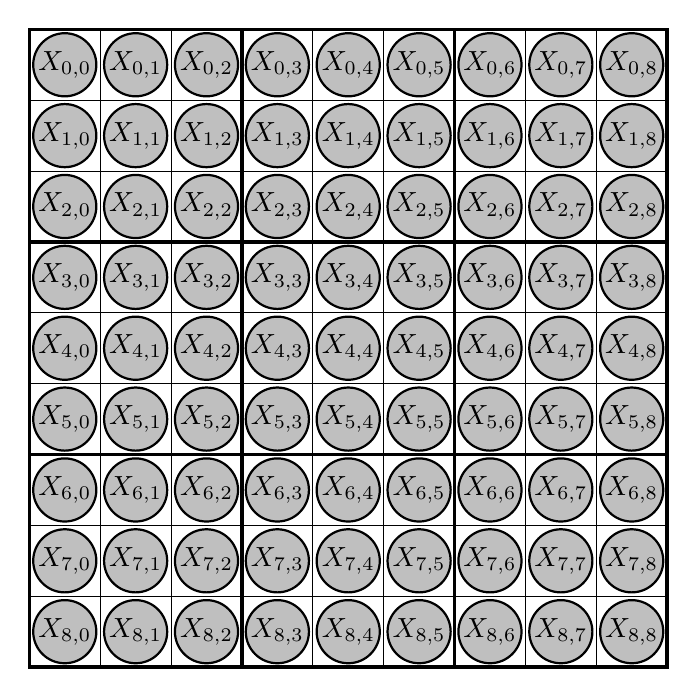
\begin{tikzpicture}[scale=0.9]
% Draw the main grid

%\node[anchor=center] (text) at (0,9) {${a)}$};

\draw[very thick] (0,0) rectangle (9,9); % Outer border
\foreach \x in {1,2,...,8} {
    \draw[thin] (\x,0) -- (\x,9); % Vertical lines
    \draw[thin] (0,\x) -- (9,\x); % Horizontal lines
}
% Thicker lines for 3x3 subgrids
\foreach \x in {3,6} {
    \draw[very thick] (\x,0) -- (\x,9); % Vertical thick lines
    \draw[very thick] (0,\x) -- (9,\x); % Horizontal thick lines
}

% Add variables in the middle of each square
\foreach \i in {0,1,...,8} {
    \foreach \j in {0,1,...,8} {
        \node[circle, draw, thick, fill=gray!50, inner sep = 0.5pt, minimum size=0.6cm, align=center] 
        at (\j+0.5,8-\i+0.5) {$X_{\i,\j}$};
    }
}

%\begin{scope}[shift={(2,0)}]
%
%\node[anchor=center] (text) at (9,9) {${b)}$};
%	
%% Draw a line of variables (horizontal)
%\foreach \k in {0,1,...,8} {
%    \node[circle, draw, thick,  fill=gray!50, inner sep=0pt, 
%    minimum size=0.6cm, align=center] 
%    at (10+\k,8.5) {$X_{i,\k}$};
%}
%
%\node[anchor=center] (text) at (9,7) {${c)}$};
%
%% Draw a column of variables (vertical)
%\foreach \l in {0,1,...,8} {
%    \node[circle, draw, thick, fill=gray!50, inner sep=0pt, 
%    minimum size=0.6cm, align=center] 
%    at (10,-\l+6) {$X_{\l,j}$};
%}
%
%\node[anchor=center] (text) at (9,7) {${d)}$};
%
%% Draw a square of variables (3x3)
%\foreach \i in {0,1,2} {
%    \foreach \j in {0,1,2} {
%        \node[circle, draw, thick, fill=gray!50, inner sep=0pt, 
%        minimum size=0.6cm, align=center] 
%        at (12+\j,6-\i) {$X_{\i,\j}$};
%    }
%}
%
%\end{scope}

\end{tikzpicture}

	\end{center}
	\caption{
	Sudoku grid of basic categorical variables $\catvariableof{i,j}$, here drawn in the standard case of $n=3$, each with dimension $\catdim=n^2=9$.
	Each basic categorical variables has $n^2$ corresponding atomization variables, which are further atomization variables to the row, column and squares constraints.
	Instead of depicting those constraints by hyperedges in a variable dependency graph, we here just indicate their existence through row, column and squares blocks.
	}
	\end{figure}

	\red{Reasoning by Entailment propagation! 
	Also, probabilistic choices possible when exact (!) contraction at a position not a basis vector, then can choose one possibility.}

\end{example}



\subsection{Hybrid Logic Network}

Markov Logic Networks are by definition positive distributions.
In contrary, Hard Logic Networks model uniform distributions over model sets of the respective Knowledge Base and therefore have vanishing coordinates.
We now show how to combine both approaches by defining Hybrid Logic Networks, when understanding Hard Logic Networks as base measures.
This trick is known to the field of variational inference, see for Example~3.6 in \cite{wainwright_graphical_2008}. 

\begin{definition}\label{def:hln}
	Given a set of formulas $\softformulaset$ with weights $\canparam$ and set $\hardformulaset$ of formulas, which conjunction is satisfiable, the hybrid logic network is the probability distribution
	\begin{align*}
		\probtensorof{(\softformulaset,\canparam,\hfbasemeasure)}[\shortcatvariables] 
		= \normationof{
		\{\exformula : \exformula\in\hardformulaset\} \cup \{\expof{\weightof{\exformula}\cdot\exformula} : \exformula\in\softformulaset\}
		}{\shortcatvariables} \, ,
	\end{align*}
	which is the member of the exponential family with statistic by $\softformulaset$ and the base measure
		\[ \hfbasemeasure[\shortcatvariables] = \contractionof{\{\formula : \formula \in \hardformulaset\}}{\shortcatvariables} \, .\]
		
	Given a set of formulas $\formulaset$, we define the set of hybrid logic networks realizable with $\formulaset$ and elementary activation cores as
	\begin{align*}
		\hlnsetof{\formulaset} 
		= \bigcup_{\secformulaset\subset\formulaset \, , \, \meanparam\in\{0,1\}^{\cardof{\formulaset}}}
		\expfamilyof{\formulaset/\secformulaset,\basemeasureof{\secformulaset,\meanparam}}
	\end{align*}
	where we denote base measures
	\begin{align*}
		\basemeasureofat{\secformulaset,\meanparam}{\shortcatvariables}
		= \bigwedge_{\enumformula\in\secformulaset} \lnot^{(1-\meanparamat{\indexedselvariable})} \enumformulaat{\shortcatvariables} \, . 
	\end{align*}
\end{definition}

The assumption of a satisfiable set $\hardformulaset$ is necessary, as we show next.

\begin{theorem}
	If any only if $\bigwedge_{\formula\in\hardformulaset}\formula$ is satisfiable, the tensor 
		\[  \contractionof{
		\{\exformula : \exformula\in\hardformulaset\} \cup \{\expof{\weightof{\exformula}\cdot\exformula} : \exformula\in\softformulaset\}
		}{\shortcatvariables} \]
	is normable.
\end{theorem}
\begin{proof}
	We need to show that
	\begin{align}\label{eq:tbsWellDefinedHLN}
		\contraction{\{\exformula : \exformula\in\hardformulaset\} \cup \{\expof{\weightof{\exformula}\cdot\exformula} : \exformula\in\softformulaset\}} > 0 \, . 
	\end{align}
	Since the conjunction of $\hardformulaset$ is satisfiable we find a $\shortcatindices$ with $\formulaat{\indexedcatvariableof{[\catorder]}}=1$ for all $\exformula\in\hardformulaset$.
	Then 
	\begin{align*}
		 \contractionof{\{\exformula : \exformula\in\hardformulaset\} \cup \{\expof{\weightof{\exformula}\cdot\exformula} : \exformula\in\softformulaset\}}{\indexedcatvariableof{[\catorder]}}  
		 & = \left( \prod_{\exformula\in\hardformulaset}\formulaat{\indexedcatvariableof{[\catorder]}} \right) 
		 \cdot \left( \prod_{\exformula\in\softformulaset}\expof{\weightof{\exformula}\cdot\exformula}[\indexedcatvariableof{[\catorder]}] \right) \\
		 & =  \left( \prod_{\exformula\in\softformulaset}\expof{\weightof{\exformula}\cdot\exformula}[\indexedcatvariableof{[\catorder]}] \right) \\
		 & > 0 \, . 
	\end{align*}
	Condition \eqref{eq:tbsWellDefinedHLN} follows from this and the Hybrid Logic Network is well-defined.
\end{proof}


\subsubsection{Tensor Network Representation}

We can employ the formula decompositions to represent both probabilistic facts of the MLN and hard facts (seen as the limit of large weights).

\begin{theorem}\label{the:hybridNetworkRepresentation}
	For any hybrid logic network we have
	\begin{align*}
		\probtensorof{(\softformulaset,\canparam,\hardformulaset)}[\shortcatvariables] 
		= \normationof{
		\{\formulaccwith : \exformula\in\softformulaset\cup\hardformulaset \}
		\cup \{\tbasisat{\formulavar} : \exformula\in\hardformulaset \}
		\cup \{\actcoreofat{\exformula}{\formulavar} : \exformula\in\softformulaset \}
		}{\shortcatvariables} \, . 
	\end{align*}
\end{theorem}
\begin{proof}
	By \lemref{lem:formulaEncodingDecomposition}.
\end{proof}

% Discussion
While the statistics computing cores in the relational encoding are shared to compute the soft and the hard logic formulas, their activation cores differ.
While probabilistic soft formulas get activation cores (see Theorem~\ref{the:mlnTensorRep})
\begin{align*}
	\actcoreofat{\exformula}{\formulavar} 
	= \begin{bmatrix} 1 \\
		 \expof{\canparamat{\indexedselvariableof{}}} 
		 \end{bmatrix}[\enumformulavar] \,
\end{align*}
the hard formulas get activation cores by unit vectors
\begin{align*}
	\tbasisat{\formulavar} 
	= \begin{bmatrix} 0 \\
		 1
	 \end{bmatrix}[\enumformulavar]  \, .
\end{align*}
As shown in \secref{sec:hardLogicLimit}, the soft activation cores converge to these hard activation cores in the limit of large parameters, when imposing a local normation.
%
We further notice, that the probabilistic activation cores are trivial tensors if and only if the corresponding parameter coordinate vanishes.


%The reason for this is the Slicing Theorem, enabling the operations by both (exponentiation and selection of one slice) by the activation cores.
For an example see Figure~\ref{fig:ActivatedHeads}.

\begin{figure}[h]
\begin{center}
	\begin{tikzpicture}[scale=0.35, thick, yscale=-1] % , baseline = -3.5pt


\draw[<-] (0,-1)--(0,1) node[midway,left] {\tiny $\catvariableof{a}$}; 
\draw[<-] (1.5,-1)--(1.5,1) node[midway,right] {\tiny $\catvariableof{b}$}; 
\draw[<-] (3,-1)--(3,1) node[midway,right] {\tiny $\catvariableof{c}$}; 
\draw (-1,-1) rectangle (4, -3);
\node[anchor=center] (text) at (1.5,-2) {$\partitionfunction \cdot \probtensor$};



\node[anchor=center] (text) at (5.5,-2) {${=}$};


\begin{scope}[shift={(11,0)}]

\draw[->] (0,1)--(0,-1)  node[midway,left] {\tiny $\catvariableof{a}$}; 
\draw[->]  (3,1)--(3,-1) node[midway,right] {\tiny $\catvariableof{b}$}; 
\draw[->] (6,1)--(6,-1) node[midway,right] {\tiny $\catvariableof{c}$}; 
	
\draw (-1,-1) rectangle (4, -3);
\node[anchor=center] (text) at (1.5,-2) {$\bencodingof{\lor}$};

\draw[->] (1.5,-3) --(1.5,-4.5) node[midway,right]{\tiny $\catvariableof{a \lor b}$};
\drawvariabledot{1.5}{-4.5}
\draw[->] (1.5,-4.5) --(1.5,-6) ;


\draw[fill, \probcolor] (1.5,-4.5) circle (0.15cm);
\draw[\probcolor] (1.5,-4.5) -- (-0.25,-4.5);
\draw[\probcolor]  (-6.75, -3.5) rectangle (-0.25, -6.5);
\node[anchor=center,\probcolor] (text) at (-3.5,-5) {$\begin{bmatrix} 
1 \\
\expof{\canparam}
\end{bmatrix}$};

\draw (5,-1) rectangle (7, -3);
\node[anchor=center] (text) at (6,-2) {$\bencodingof{\lnot}$};

\draw[->] (6,-3) --(6,-4.5) node[midway,right]{\tiny $\catvariableof{\lnot c}$};
\drawvariabledot{6}{-4.5}
\draw[->] (6,-4.5) --(6,-6);	


	
\draw (0.5,-6) rectangle (6.5,-8);
\node[anchor=center] (text) at (3.5,-7) {$\bencodingof{\lor}$};
	
\draw[<-] (4,-9.5) -- (4,-8) node[midway,right] {\tiny $\catvariableof{a \lor b \lor \lnot c}$};

\draw[fill,\concolor] (4,-9.5) circle (0.15cm);
\draw[\concolor] (4,-9.5) -- (2.25,-9.5);
\draw[\concolor]  (0.25, -8.5) rectangle (2.25, -11.5);
\node[anchor=center,\concolor] (text) at (1.25,-10) {$\begin{bmatrix} 
0 \\
1
\end{bmatrix}$};

%\draw (3,-9) rectangle (5,-11);
%\node[anchor=center] (text) at (4,-10) {$\truevectorat{}$};

\end{scope}

\end{tikzpicture}
\end{center}
\caption{Diagram of a formula tensor with activated heads, containing \textcolor{\concolor}{hard constraint cores} and \textcolor{\probcolor}{probabilistic weight cores} .} %along \textcolor{\inactivecolor}{inactive cores}.}
\label{fig:ActivatedHeads} 
\end{figure}



\begin{remark}{Probability interpretation using the Partition function}
	The tensor networks here represent unnormalized probability distributions.
	The probability distribution can be normed by the quotient with the naive contraction of the network, the partition function.
\end{remark}


\subsubsection{Reasoning Properties}

Deciding probabilistic entailment (see \defref{def:probEntailment}) with respect to Hybrid Logic Networks can be reduced to the hard logic parts of the network.

\begin{theorem}\label{the:hlnEntailmentReduction}
	Let $(\softformulaset,\canparam,\hardformulaset)$ define a Hybrid Logic Network.
	Given a query formula $\exformula$ we have that 
		\[ \probtensorof{(\softformulaset,\canparam,\hardformulaset)} \models \exformula \]
	if and only if
		\[ \hardformulaset \models \exformula \, . \]
\end{theorem}
\begin{proof}
	This follows from Theorem~\ref{the:factorReduction} on the representation of Hybrid Logic Networks as Markov Networks in Theorem~\ref{the:hybridNetworkRepresentation}.
\end{proof}


Formulas in $\softformulaset$, which are entailed or contradicted by $\hardformulaset$ are redundant, as we show next.

\begin{theorem}%\label{the:hlnRepRedundancy}
	If for a formula $\exformula$ and $\hardformulaset$ we have 
		\[ \hardformulaset \models \exformula \, \quad \text{or} \quad \hardformulaset \models \lnot\exformula \]
	then for any $(\softformulaset,\canparam,\hardformulaset)$
		\[ \probofat{(\softformulaset/\{\exformula\},\tilde{\canparam},\hardformulaset)}{\shortcatvariables} =  \probofat{(\softformulaset,\canparam,\hardformulaset)}{\shortcatvariables}  \, , \]
	where $\tilde{\canparam}$ denotes the tensor $\canparam$, where the coordinate to $\exformula$ is dropped, if $\exformula\in\softformulaset$.
\end{theorem}
\begin{proof}
	Isolate the factor to the hard formula, which is constant for all situations.
\end{proof}

%% Now in the 
A similar statement holds for the hard formulas itself, as shown in Theorem~\ref{the:ReduncancyOfEntailed}.
However, notice that if $\hardformulaset/\{\exformula\}\models\lnot\exformula$, then $\hardformulaset\cup\{\exformula\}$ is not satisfiable and a hybrid logic network cannot be defined for $\hardformulaset\cup\{\exformula\}$ as hard logic formulas.

%If the conjunction of $\hardformulaset/\{\exformula\}$ entails $\exformula$, we can erase $\exformula$ from $\hardformulaset$ without changing the contraction, therefore without changing the base measure of the Hybrid Logic Network.

% Utility in Contraction KB implementation
These results are especially interesting for the efficient implementation of Algorithm~\ref{alg:TensorKB}, which has been introduced in \charef{cha:logicalReasoning}.
By Theorem~\ref{the:hlnEntailmentReduction} only the hard logic parts of a Hybrid Logic Network are required in the ASK operation.
%Theorem~\ref{the:hlnRepRedundancy} for the TELL operation, but already discussed in more generality

\subsubsection{Expressivity}

Hybrid Logic Networks extend the expressivity result of Theorem~\ref{the:mintermExpressivityMLN} to arbitrary probability tensors, dropping the positivity constraints for Markov Logic Networks.

\begin{theorem}\label{the:mintermExpressivityHLN}
	Let $\probat{\shortcatvariables}$ a possibly not positive probability tensor we build a base measure
		\[ \hfbasemeasure = \nonzeroof{\probat{\shortcatvariables}} \]
	and a parameter tensor
	\begin{align*}
		\canparamat{\selvariableof{[\catorder]}=\shortcatindices}
		= \begin{cases}
			0 & \text{if} \quad \probat{\indexedshortcatvariables} = 0  \\
			\lnof{\probat{\indexedshortcatvariables}} & \text{else} 
		\end{cases} \, . 
	\end{align*}
	Then the probability tensor is the member of the minterm exponential family with base measure $\hardformulaset$ and parameter $\canparam$, that is
		\[ \probat{(\mintermformulaset,\canparam,\hfbasemeasure)}\]
\end{theorem}
\begin{proof}
	It suffices to show that 
		\[ \sbcontractionof{\hfbasemeasure, \expof{\contractionof{
		\sencodingof{\mintermformulaset}\canparam
		}{
		\shortcatvariables
		}}}{\shortcatvariables} = \probat{\shortcatvariables} \, . \]
	For indices $\shortcatindices$ with $\probat{\indexedshortcatvariables}=0$ we have $\hfbasemeasureat{\indexedshortcatvariables}=0$ and thus also 
		\[ \sbcontractionof{\hfbasemeasure, \expof{\contractionof{
		\sencodingof{\mintermformulaset}\canparam
		}{
		\shortcatvariables
		}}}{\indexedshortcatvariables} = 0 \, . \]
	For indices $\shortcatindices$ with $\probat{\indexedshortcatvariables}>0$ we have $\hfbasemeasureat{\indexedshortcatvariables}=1$ and
	\begin{align*}
		 \sbcontractionof{\hfbasemeasure, \expof{\contractionof{
		\sencodingof{\mintermformulaset},\canparam
		}{
		\shortcatvariables
		}}}{\indexedshortcatvariables} 
		&= \prod_{\selindexof{[\catorder]}} \expof{\canparamat{\selvariableof{[\catorder]}=\selindexof{[\catorder]}} \cdot \mintermofat{\selindexof{[\catorder]}}{\indexedshortcatvariables}} \\
		&=  \expof{\canparamat{\selvariableof{[\catorder]}=\shortcatindices}} \\
		&=  \probat{\indexedshortcatvariables} \, .
	\end{align*}
\end{proof}

\subsection{Applications}

Hybrid Logic Networks as neuro-symbolic architectures:
\begin{itemize}
	\item Neural Paradigm here by decompositions of logical formulas into their connectives.
		In more generality by decompositions of sufficient statistics into composed functions, using Basis Calculus.
		Deeper nodes as carrying correlations of lower nodes.
	\item Symbolic Paradigm by interpretability of propositional logics.
\end{itemize}


Hybrid Logic Networks as trainable Machine Learning models:
\begin{itemize}
	\item Expressivity: Can represent any positive distribution, as shown by Theorem~\ref{the:maximalClausesRepresentation}, with $2^d$ formulas.
	\item Efficiency: Can only handle small subsets of possible formulas, since their possible number is huge.
		Tensor networks provide means to efficiently represent formulas depending on many variables and reason based on contractions.
	\item Differentiability: Distributions are differentiable functions of their weights, see Parameter Estimation Chapter. 
		The log-likelihood of data is therefore also differentiable function of their weights and we can exploit first-order methods in their optimization.
	\item Structure Learning: We need to find differentiable parametrizations of logical formulas respecting a chosen architecture.
		In \charef{cha:formulaBatches} such representations are described based on Selector Tensor Networks.
\end{itemize}
Differentiability and structure learning will be investigated in more detail in the next chapter.

\red{When understanding atoms as observed variables, and the computed as hidden, Hybrid Logic Networks are deep higher-order boltzmann machines: 
More generic correlations can be captured by a logical connective, calculated by a relational encoding and activated by an activation core.}

\red{Hybrid Logic Networks as bridging soft and hard logics within the formalism of exponential families.}

%\begin{remark}[Hopfield networks]
%	Also interesting for MLNs is a Hopfield perspective.
%	Having an initialization the update can be interpreted as a Gibbs sampling step at temperature $0$ (since deterministic update).
%\end{remark}


% CSP
A more general class of problems, which have natural representations by Hard Logic Networks are Constraint Satisfaction Problems (see Chapter~5 in \cite{russell_artificial_2021}).
Solving such problems is then equivalent to sampling from the worlds in a logical interpretation, and can be approached by the methods of \charef{cha:logicalReasoning}.
Among these classed, we have only discussed the Sudoku game in Example~\ref{exa:sudoku}.
Extensions by Hybrid Logic Networks can be interpreted as implementations of preferences among possible solutions by probabilities.




